\chapter{Lab 2: Basic Programming}

This chapter follows chapter 3 of \citet{R:Jones:2009}.

\section{Topics}

\begin{itemize}
\item writing scripts
\item sourcing
\item if else
\end{itemize}

\section{Writing scripts}


When typing many commands at the R command line it quickly becomes
cumbersome to keep track of computations and logic of the code. Thus,
it is more efficient to write the code in a separate file which we
will call script. The extension normally used for R extensions is
\texttt{.r}. Since it is possible that previous objects were created
in an R session, we can first choose to clean the workspace using the
\texttt{rm(list=ls())} command. A simple script can be as follows

\begin{lstlisting}
## Converting from Fahrenheit (F) to Celsius (C)
## First eliminate existing objects in the workspace
rm(list=ls())

## Use some input values
x1 <- 40
x2 <- 50
x3 <- 70
x4 <- 80

## Convert these values to Celsius
## The formula is C = (F - 32) * 5/9

x1.C <- (x1 - 32) * 5/9
x2.C <- (x2 - 32) * 5/9
x3.C <- (x3 - 32) * 5/9
x4.C <- (x4 - 32) * 5/9

## Original values
print(c(x1, x2, x3, x4))

## Celsius values
print(c(x1.C, x2.C, x3.C, x4.C))

\end{lstlisting}

If we save this file as \texttt{far-cel.r} we can execute it at the R
command line

\begin{lstlisting}
> source("far-cel.r")
[1] 40 50 70 80
[1]  4.44 10.00 21.11 26.67
\end{lstlisting}

This assumes that the script is in the same directory (or folder) as
the current working directory (\texttt{getwd()}). At the end of lab
you will have an opportunity to improve this script.

\subsection{Control Flow}

Let us say that we are given some temperature data and we want to
convert from F to C but we are not sure whether the input is in F or
not. For problems like this we can sometimes use programming
statements such as \texttt{if} and \texttt{else}. For example

\begin{lstlisting}
## Convert x from F to C if input is in F

x <- 50

units <- "F"

if(units == "F"){
  x <- (x - 32) * 5/9
}

\end{lstlisting}

At this point the previous code might not make a lot of sense, but it
serves to illustrate the if statement and it shows how we started with
one object (\texttt{x}) which contained temperature in the F scale and
then replaced that value with temperature in the C scale. Notice that
although many times we use an \texttt{if} together with an
\texttt{else} the else part is optional. Also the basic construct of
an \texttt{if} statement is as follows

\begin{lstlisting}
if(logical_expression){
   expression_1
   expression_2
   ...
}else{
   expression_n
   expression_n+1
   ...
}
\end{lstlisting}

The brackets \texttt{\{\}} are used to combine several statements with
the \texttt{if, else} clause.

In many programs it is necessary to create a loop. This can be
accomplished with the \texttt{for} command

\begin{lstlisting}
for(x in vector){
   expression_1
   expression_2
   ...
}
\end{lstlisting}

As an example we can compute the cumulative sum of the first 10 integers

\begin{lstlisting}

sum_x <- 0
for(i in 1:10){
   sum_x <- sum_x + i
   cat("the current loop element is ",i,"\n")
   cat("the current cumulative sum is ",sum_x,"\n")
}
## Executing this code produces
the current loop element is  1 
the current cumulative sum is  1 
the current loop element is  2 
the current cumulative sum is  3 
the current loop element is  3 
the current cumulative sum is  6 
the current loop element is  4 
the current cumulative sum is  10 
the current loop element is  5 
the current cumulative sum is  15 
the current loop element is  6 
the current cumulative sum is  21 
the current loop element is  7 
the current cumulative sum is  28 
the current loop element is  8 
the current cumulative sum is  36 
the current loop element is  9 
the current cumulative sum is  45 
the current loop element is  10 
the current cumulative sum is  55 
\end{lstlisting}

The \texttt{for} command is not the only way to create a loop. There
is also the \texttt{while} command

\begin{lstlisting}
while(logical_expression){
     expression_1
     expression_2
     ...
}
\end{lstlisting}

The statements inside the brackets will be executed until the
condition in the while statement becomes false. This should be done
with caution as the condition is never falsified we will end up
creating an infinite loop.

As an example we can look at the Fibonacci series. In botany it
appears, for example, in the disposition of flowers in a head of
sunflower \citep{Thornley:2000}. The Fibonacci sequence is defined as
$F_1 = 1$, $F_2 = 1$, and $F_n = F_{n-1} + F_{n-2}$ for $n \geq 2$. We
can find the first \texttt{x} Fibonacci numbers

\begin{lstlisting}
## Calculate the first x Fibonacci numbers

## Clear the workspace
rm(list=ls())

## Set x equal to 100
x <- 100

## Initialize variables
F <- c(1, 1)
n <- length(F)

while(F[n] <= 100){
      cat("n = ",n," F[n] = ",F[n], "\n")
      n <- n + 1
      F[n] <- F[n - 1] + F[n - 2]
}
\end{lstlisting}

\subsection{Vector-based programming}

In R it is generally more efficient to use what is called vectorized
operations. These tend to be shorter and more computationally
efficient.

For example, we can find the sum of the first 100 squares using a loop

\begin{lstlisting}
> n <- 100
> S <- 0
> for(i in 1:n){
+     S <- S + i^2
> }
> S
[1] 338350
\end{lstlisting}

Using vector operations this is simply

\begin{lstlisting}
> S <- sum((1:n)^2)
[1] 338350
\end{lstlisting}

This one line needs to be broken down to understand what is going
on. First, a sequence from 1 to 100 was created \texttt{1:n}, then the
squaring is applied to each element (i.e. it is vectorized). Finally,
all the 100 elements squared are added up and stored in an object
\texttt{S}. The result is the same.

\subsection{Program flow}

It is an useful exercise to study how the variables change through a
program and how the different steps are executed. From
\citet{R:Jones:2009} we have a nice example of flow control, Figure
\ref{fig:r-flow}.


\begin{figure}[htpb!]
  \centering
  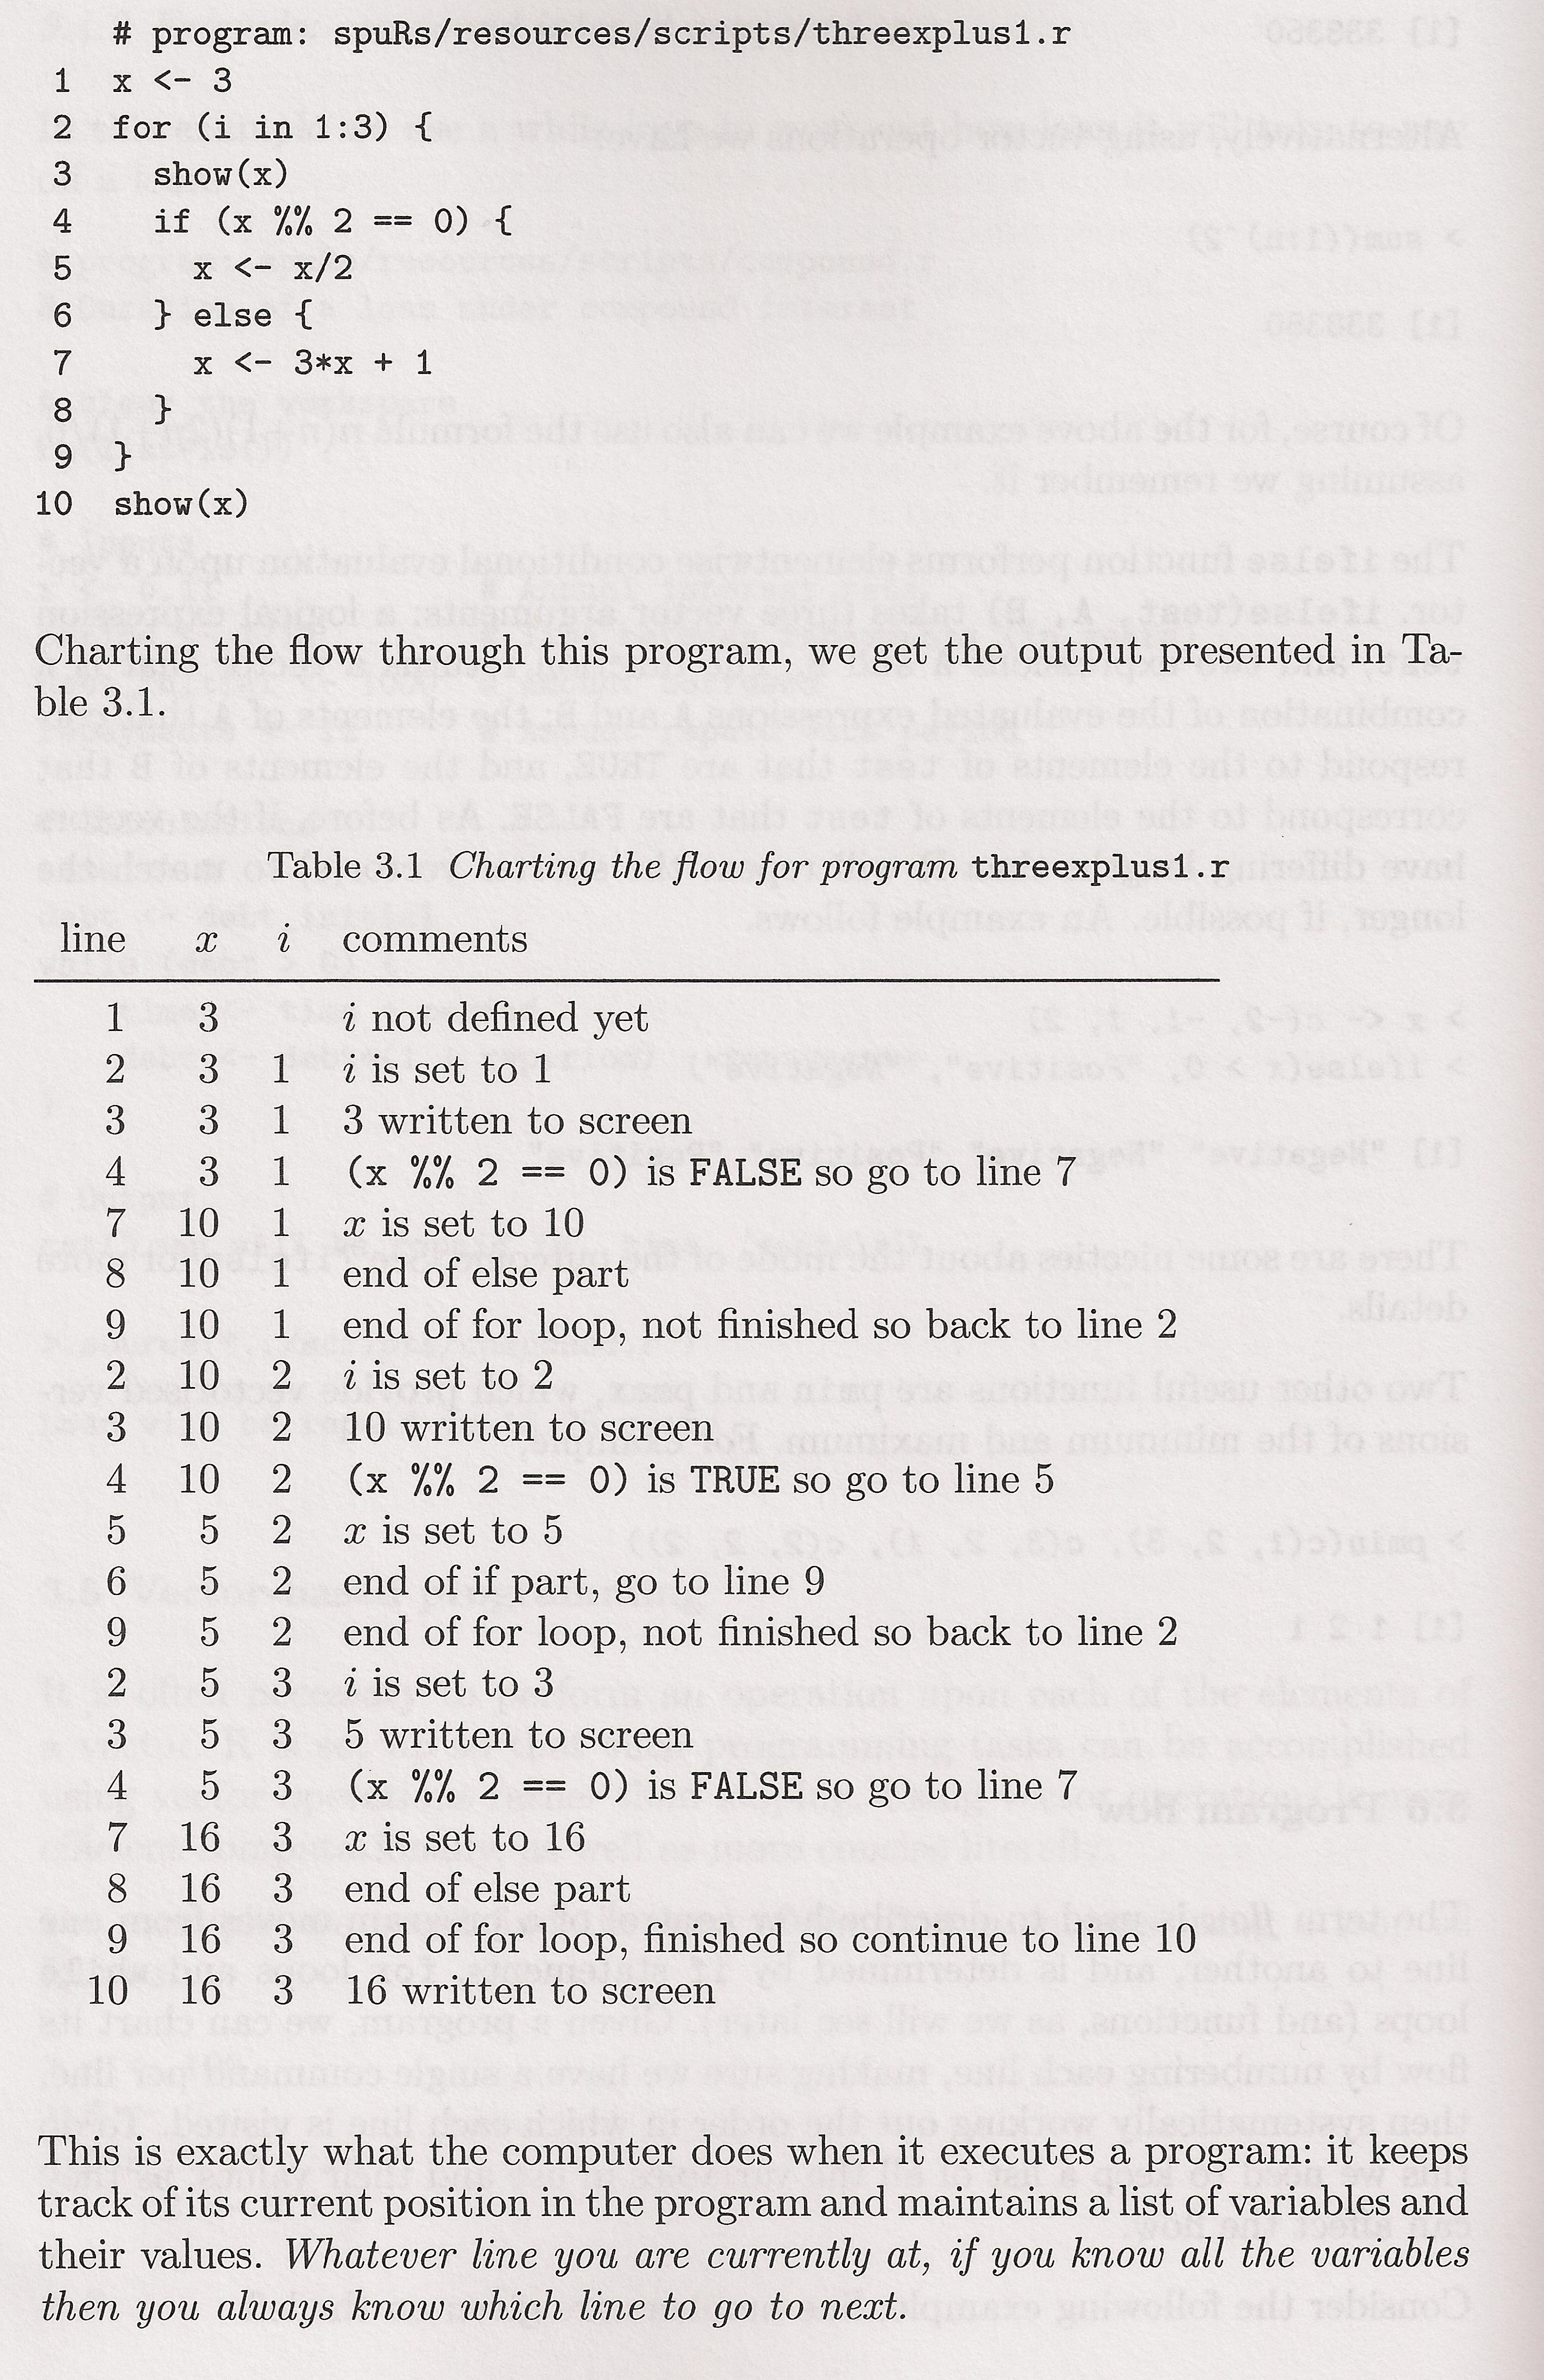
\includegraphics[scale=0.11]{./ch_04/figs/r-flow.png}
  \caption{Scanned page from \citet{R:Jones:2009} illustrating program flow.}
  \label{fig:r-flow}
\end{figure}

\section{Programming with functions}

This is similar to chapter 5 of \citet{R:Jones:2009}.

``Functions are one of the main building blocks of large programs and
they are an essential tool for structuring complex algorithms. In
some other languages \emph{procedures} and \emph{subroutines} play the
same role as functions in R.''

\subsection{Functions}

A function has the form 

\begin{lstlisting}
fname <- function(argument_1, argument_2, ...){
                 expression_1
                 expression_2
                 ...
                 return(output)
}
\end{lstlisting}

The function is run by simply

\begin{lstlisting}
fname(x1, x2, ...)
\end{lstlisting}

We say here that \texttt{x1} and \texttt{x2} are passed to the
arguments of the function. Let us say we write a very simple function
to add to values.

\begin{lstlisting}
## Creating functions
add2values <- function(x, y){

  result <- x + y

  return(result)

}
\end{lstlisting}

This is, of course, a trivial function but it illustrates the basic
building blocks of writing a function. The return statement is
optional, so the same can be achieved with the following

\begin{lstlisting}
## Creating functions
add2values <- function(x, y){

  result <- x + y

  result

}
\end{lstlisting}

Going back to section \ref{ch-intro:desc-model} and equation
\ref{ch-intro:eq-poly}. We can write this polynomial as an R function.

\begin{lstlisting}
poly3 <- function(x, beta0, beta1, beta2, beta3){

  y <- beta0 + x * beta1 + x^2 * beta2 + x^3 * beta3

  y

}
\end{lstlisting}

Similarly, we can turn to Eq. \ref{eq:logis} and build an R function (without
the error term). It is important to notice that we need to run these
function so that they appear in the R workspace.

\begin{lstlisting}
## A function for a logisitc model
logistic <- function(x, Asym, xmid, scal){

  y <- Asym / (1 + exp((xmid - x)/scal))
  y

}
\end{lstlisting}

We can run the \texttt{ploy3} equation with some arguments

\begin{lstlisting}
x <- 1:10
res <- poly3(x, 3, 2, 0.5)
Error in x^3 * beta3 : 'beta3' is missing
\end{lstlisting}

Notice that we only provided values for \texttt{beta0},
\texttt{beta1}, \texttt{beta2}, but not for \texttt{beta3}. R prints
an error saying that there is no value assigned to \texttt{beta3} and
thus cannot complete the operation.

\begin{lstlisting}
## Second try
x <- 1:10
res <- poly3(x, 3, 2, 0.5, 0.1)
\end{lstlisting}

To visualize the results we can use the \texttt{plot} command.

\begin{lstlisting}
## Visualizing results
plot(x, res)
\end{lstlisting}

We can run the logistic function and display the results together

\begin{lstlisting}
## Running the logisitc function
res2 <- logistic(x, 150, 5, 2)

## Adding the result to the previous plot
plot(x, res)
points(x, res2, pch = 15)
\end{lstlisting}

\section{Exercises}

\begin{enumerate}
\item Improve the script \texttt{far-cel.r} by creating a function.
\item Write a cumulative sum function for an arbitrary vector using
  the \texttt{for} command. Note that the \texttt{cumsum} function
  does this.
\item Write a function that calculates growing degree days.

\end{enumerate}